% JKAIA 2026 (2026 한국인공지능학회 추계학술대회) -- General (Poster) 트랙, 논문 A 한국어 작업본
% ※ 제출본은 영문 main.tex다. 이 파일은 저자가 내용을 검토·수정하기 위한 한국어 대조본이며, 문단 구조가 main.tex와 1:1로 같다.
%    이 파일을 고치면 같은 자리의 영문을 main.tex에 반영한다.
% 템플릿: kaia.cls (포스터 트랙 공식 ZIP, 2026-10-01 이후 바뀌지 않음을 2026-10-24에 확인). 포스터 트랙은 이 템플릿으로 1~2쪽 요약본을 낸다.
% 심사는 single-blind이므로 저자를 명기한다. 학회 안내: "제출 논문은 영문으로 작성" → 영문 main.tex를 제출한다.
% 모든 수치는 ../../main/results에서 다시 계산했다(2026-10-24). 출처는 ../README.md에 있다.
%
% 빌드: tectonic -X compile main_ko.tex  (XeTeX: 한글은 kotex + Apple SD Gothic Neo)
%
% 템플릿 대비 변경점(main.tex와 같음):
%  * 템플릿의 \fbox{\parbox}는 쪽을 넘기지 못하므로 두 쪽 요약을 위해 mdframed로 같은 테두리를 그린다.
%  * kaia.cls의 \maketitle이 \twocolumn[...]을 호출하므로 \twocolumn을 1단으로 재정의해 템플릿 PDF와 같은 1단을 유지한다.
%  * XeTeX에서는 Times(mathptmx)가 매핑되지 않아 시스템 Times New Roman을 쓴다.

\documentclass[nouppercase]{kaia}
\usepackage{amsmath}
\usepackage{booktabs}
\usepackage{graphicx}
\usepackage[framemethod=TikZ]{mdframed}
\usepackage{iftex}
\ifXeTeX
  \usepackage{fontspec}
  \setmainfont{Times New Roman}
  \usepackage{kotex}
  \setmainhangulfont{Apple SD Gothic Neo}[BoldFont={* Bold}, ItalicFont={* Light}]
\else
  \usepackage{kotex}
\fi
\AtBeginDocument{\hypersetup{hidelinks}}
\graphicspath{{figures/}}

\makeatletter
\renewcommand{\twocolumn}[1][]{#1}   % 1단 유지; \maketitle의 선택 인자는 그대로 조판된다
\makeatother
\mdfsetup{linewidth=0.4pt, linecolor=black, innerleftmargin=7pt, innerrightmargin=7pt,
          innertopmargin=4pt, innerbottommargin=4pt, skipabove=4pt, skipbelow=4pt}
\newcommand{\shiter}{\textsf{sh-iter}}
\newcommand{\dtm}{\textsf{det}}
\renewenvironment{abstract}{\center\textbf{\large{요약}}\par\vspace{0.5\baselineskip}\begin{quote}}{\end{quote}}  % kaia.cls hard-codes "Abstract"

\title{계획기는 결정적 오차를 이용한다: 저비트 월드모델을 위한 dither\\[2pt]
{\normalsize\normalfont Planners Exploit Deterministic Error: Dithered Low-Bit World Models}}

\author{송용휘}{a}
\author{이건명}{b}
\affiliation{충북대학교 정보통신공학부, 대한민국, thddydgnl1937@gmail.com}{a}
\affiliation{충북대학교 소프트웨어학부, 대한민국, kmlee@cbnu.ac.kr}{b}

\begin{document}

\maketitle
\vspace{-28pt}

\begin{mdframed}

\begin{abstract}
MPPI와 CEM 같은 표본 기반 계획기는 결정 한 번에 월드모델을 수천 번 호출한다. 그런데 저비트 월드모델이 계획에서 실패하는 정도는 비트 수나 1-step 예측 오차로 설명되지 않는다. 본 연구는 손상을 정하는 것이 반올림 오차의 크기가 아니라 구조임을 보인다. 결정적 반올림(round-to-nearest)은 최적화 반복 내내 그대로 남는 오차장을 만들고, 기전을 검정한 네 과제에서 반복형 계획기는 이 오차장이 우연히 유리하게 평가하는 후보 쪽으로 이동했다. 같은 비트 수에서 학습 없이 반올림만 dither(확률적 반올림)로 바꾸고, 그 잡음을 모든 후보가 공유하며 계획기 반복마다 새로 뽑으면 이 이동의 대부분이 사라진다. TD-MPC2(MPPI, 12과제)와 DINO-WM(CEM, 3과제)으로 내부 사전등록한 실험에서 결정적 반올림은 성공률을 최대 100퍼센트포인트 떨어뜨렸지만, 손상이 실재한 36칸 중 29칸에서 그 1-step 오차는 dither보다 크지 않았다. dither는 Meta-World 손상 칸 19개 모두에서 손상의 절반 이상(중앙값 95퍼센트)을, DINO-WM 5칸 중 4칸에서 절반 이상을 없앴고, TD-MPC2의 융합 정수 kernel에서 추가 지연의 중앙값은 10퍼센트 미만이었다. 이 처방은 반복하는 계획기가 필요하고, 유리한 오차가 반복 사이에 덜 지속되는 DMC 같은 과제에서는 효과가 작다.
\end{abstract}
\begin{keywords}
월드모델, 모델 예측 제어, 양자화, 확률적 반올림, 로봇 계획
\end{keywords}

\subsection{문제 설정}
MPC 계획기는 결정 한 번에 월드모델을 후보 수 $\times$ 반복 수 $\times$ horizon만큼 호출한다. TD-MPC2~[1]의 MPPI는 $512\times6\times3$번, PushT에서 DINO-WM~[2]의 CEM은 $300\times30\times5$번이다. 저비트 추론은 이 비용을 줄이는 가장 직접적인 방법이지만, 양자화한 월드모델은 비트 수나 오프라인 오차로 설명되지 않는 방식으로 계획을 망가뜨린다~[3, 4]. 본 연구는 MLP 은닉 활성(TD-MPC2의 dynamics·reward 층 4개, DINO-WM의 예측기 블록 6개)을 보정한 균일 격자 위에서 $k$비트로 양자화한다. 과제마다 사전등록한 규칙이 held-out episode에서 $k$를 고르고(주로 round-to-nearest, 즉 \dtm{}가 20\%p 이상 잃는 가장 큰 $k$), $k-1$, $k$, $k+1$을 시험한다. 질문은 두 가지다. \dtm{}는 왜 1-step 오차가 말해 주는 것보다 계획을 더 망가뜨리는가? 반올림만 바꾸면 이를 고칠 수 있는가?

\subsection{새로운 점}
(1) \textit{이용의 직접 측정.} 계획기 이용 지수(OEI)는 실행된 계획의 모델 비용 오차에서 첫 반복 무작위 후보의 오차를 뺀 값이다. 이 값은 선택 항과 이동 항으로 정확히 나뉜다. (2) \textit{2축 대조}: 항목별 오차 분포는 같고, 후보 간 공유 여부와 반복 간 지속 여부만 다른 확률적 변형들을 비교한다. (3) \textit{같은 비트 수에서 학습 없이 쓰는 처방}(\shiter). 저비트 월드모델이나 VLA 추론에 dither나 확률적 반올림을 쓴 선행연구는 찾지 못했다. 가장 가까운 연구~[5]는 후보 공통 오차와 행동 상대 오차를 oracle 수리로 나누지만, 반복 축, 압축 오차, 배치 가능한 처방이 없다. 처방의 원리인 optimizer's curse~[6], 공통 난수, 확률적 반올림~[7]은 고전적이다. 새로운 것은 이를 압축된 월드모델에 적용한 것, 두 축을 분리한 것, 효과의 크기다. (4) \textit{내부 사전등록}: 가설, 문턱, 코드를 단계마다 시각을 기록한 문서로 미리 고정했고, 성립하지 않은 가설도 보고한다(표~\ref{tab:hyp}).

\subsection{알고리즘}
\textbf{반올림 변형.} 격자 간격이 $\Delta$일 때 \dtm{}는 $x$를 $\Delta\,\mathrm{round}(x/\Delta)$로, dither는 $u\sim U[0,1)$로 $\Delta\lfloor x/\Delta+u\rfloor$로 바꾼다. dither는 편향이 없다. 확률적 변형들은 $u$를 뽑는 방식만 다르다. 후보마다 따로 뽑거나(\textsf{ind}), 모든 후보가 공유하고 forward 호출마다 새로 뽑아 계획기 반복마다 새롭게 하거나(\shiter, 처방), 공유하되 한 제어 step(\textsf{sh-step}) 또는 한 episode(\textsf{sh-ep}) 동안 고정한다(open-loop CEM에서는 둘이 같다). 나머지 계획기 설정은 공식값이다(MPPI: elite 64; CEM: top 30, Wall·PointMaze는 반복 10회).
\textbf{이용.} 후보 $a$의 비양자화 모델 대비 비용 오차를 $e(a)$라 하면 $\mathrm{OEI}=e(a_{\mathrm{exec}})-\bar e_{\mathrm{first}}=\text{선택}+\text{이동}$이다. 이동은 모집단 평균 오차가 첫 반복에서 마지막 반복까지 바뀐 양이다. 이동이 음수이면 계획기가 오차가 유리한 후보 쪽으로 움직였다는 뜻이다.
\textbf{이론.} 새로 뽑는 무편향 잡음의 이동 기대값은 0이다. 반면 지속되는 오차장은 모집단을 평활한 모델 비용의 최소점으로 끌고 간다(표본평균근사 편향). 유도한 선택·이동 항은 MPPI·CEM 모의 92만 2천 회와 맞았다(맞춘 기울기 0.92--1.05).

\begin{center}
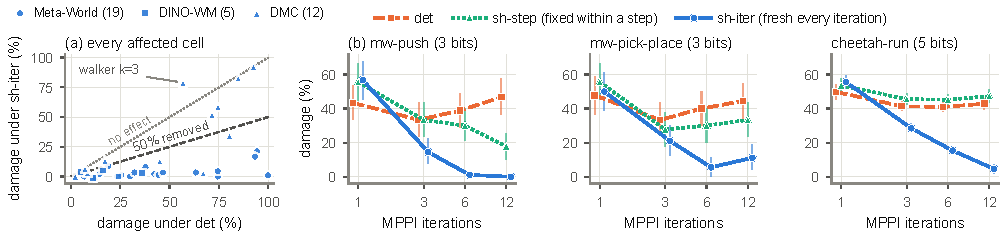
\includegraphics[width=\linewidth]{fig_main.pdf}
\captionof{figure}{(a) 모든 손상 칸에서 \dtm{} 손상 대비 \shiter{} 손상(성공률 하락, DMC는 상대 return 하락). 파선 아래는 \shiter{}가 손상의 절반 이상을 없앤 칸이다. (b) MPPI 반복 수에 따른 손상(TD-MPC2, 짝 90 episode, 95\% CI).}
\label{fig:main}
\end{center}

\subsection{실험}
\textbf{설정.} TD-MPC2: 공식 5M checkpoint(seed 3개), Meta-World 8과제(성공률)와 DMC 4과제(return), 과제--비트 칸 36개, 변형마다 짝 90 episode. DINO-WM: 공식 PushT·Wall·PointMaze 모델, 9칸, 짝 100 episode. 모든 변형은 비양자화 기준선과 짝을 이루고(같은 seed와 계획기 잡음), 손상 $D$는 기준선 대비 하락이다(DMC는 상대 return). \dtm{} 하락은 과제별 Holm 보정(짝 bootstrap, 95\%)을 통과하면 실재한다고 보고, 그런 칸을 손상 칸이라 부른다(TD-MPC2 31칸, DINO-WM 5칸).
\textbf{현상과 처방}(그림~\ref{fig:main}a). \dtm{}는 성공률을 최대 100\%p 떨어뜨린다(mw-button-press, 2비트). 이 손상 칸 36개 중 29개에서 \dtm{}의 1-step 오차는 \shiter{}보다 크지 않다(mw-pick-place 3비트: 0.22 대 0.39인데, 하락은 37.8\%p 대 7.8\%p). \shiter{}는 Meta-World 손상 칸 19개 모두에서 손상의 절반 이상(중앙값 95\%)을, DINO-WM 5칸 중 4칸에서 절반 이상을 없애고, Meta-World와 DINO-WM의 손상 칸 어디에서도 \dtm{}보다 나쁘지 않다.
\textbf{기전}(그림~\ref{fig:main}b). \dtm{}에서는 기전 과제 네 개 모두에서(각 과제의 1차 비트 수) 모집단 평균 오차가 유리한 쪽으로 이동한다. \shiter{}는 그 이동의 24\% 이하만 남기고, TD-MPC2의 지속 dither는 70--130\%를 남긴다. dither의 이득은 반복이 있어야 생긴다. 반복이 1회면 \shiter{}도 \dtm{}보다 낫지 않지만, 반복 12회에서는 \shiter{} 손상이 0--11\%이고 \dtm{}는 43--47\%에 머문다. elite 수를 고정하면 후보 수가 늘수록 이용과 손상이 함께 커지고(4과제 중 3과제), 고정 dither의 손상은 독립 offset 수(표 크기)가 커질수록 줄어든다(6과제 중 5과제).
\textbf{DMC.} \dtm{}의 유리한 오차 가운데 반복 사이에 지속되는 몫(지속 몫, 이동을 OEI로 나눈 값)은 DMC에서 0.33--0.52로 Meta-World(0.54--0.73)보다 작다. TD-MPC2 12과제 전체에서 이 몫은 \shiter{}의 효과를 예측했다(Spearman 0.83, 1단계 뒤에 정하고 새 seed로 돌린 검정). DMC에서 \shiter{}는 12칸 중 5칸에서만 손상의 절반 이상을 없애고, walker 3비트에서는 오히려 해롭다(return 손실 78.9\% 대 56.9\%).

\begin{center}
\footnotesize
\setlength{\tabcolsep}{5pt}
\begin{tabular}{@{}p{0.58\linewidth}>{\raggedright\arraybackslash}p{0.38\linewidth}@{}}
\toprule
가설과 사전등록 검정 & 결과 \\
\midrule
H1: 어떤 손상 칸에서 \dtm{}의 1-step 오차 $\le$ \shiter{} & 두 계열 모두 성립 \\
H3a: 손상 칸의 75\% 이상에서 \shiter{}가 손상의 50\% 이상 제거, 5\%p 넘게 나쁜 칸 없음 & Meta-World 19/19, DINO-WM 4/5; DMC 불성립 \\
DMC 설명(1단계 뒤 추가): 지속 몫과 손상 제거율의 Spearman $\ge0.5$ & 성립: 12과제에서 0.83 \\
H2a$'$(1단계 뒤 추가): \dtm{} 이동 $<0$, 이동 비 \shiter/\dtm{} $<0.5$ & 성립: 4/4과제(비 $\le$0.24) \\
H2c: 후보 수와 $|\mathrm{OEI}_{\dtm}|$, $D_{\dtm}$의 Spearman $\ge0.8$ & 성립: 3/4과제 \\
H4a: 표 크기와 고정 dither 손상의 Spearman $\le-0.8$ & 성립: 5/6과제(셋은 정확히 $-0.8$) \\
H3b: 최선 PTQ 위에서 3--4비트 칸 과반에서 \shiter{}가 \dtm{}보다 나음 & TD-MPC2 성립(10/19); DINO-WM 불성립(1/3) \\
H5: dither 지연 오버헤드 $\le$10\%; Pareto 지배 설정 하나 이상 & 약하게 성립(최대 6.9\%); fp32보다 빠르지 않음 \\
H2a, H2b(원래 OEI 검정); H4b(near-tie 밀도와 공유 이득) & 불성립(주장을 좁힘) \\
\bottomrule
\end{tabular}
\captionof{table}{사전등록 가설과 결과. 기전 과제: mw-push, mw-pick-place, cheetah-run, PushT.}
\label{tab:hyp}
\end{center}

\par\vspace{3pt}\noindent{\scriptsize\textbf{참고문헌.}
[1]~N.~Hansen, H.~Su, X.~Wang, TD-MPC2, ICLR, 2024.
[2]~G.~Zhou et al., DINO-WM, arXiv:2411.04983, 2024.
[3]~Z.~Fu et al., An empirical study of world model quantization, arXiv:2602.02110, 2026.
[4]~J.~Xu et al., Predict before you deploy (PreDE), arXiv:2609.19441, 2026.
[5]~R.~Min et al., When low prediction error misleads planning, arXiv:2610.05550, 2026.
[6]~J.~E.~Smith, R.~L.~Winkler, The optimizer's curse, Management Science, 2006.
[7]~S.~Gupta et al., Deep learning with limited numerical precision, ICML, 2015.\par}

\end{mdframed}

\end{document}
